\chapter{Implementation Platform - Clang/LLVM}
\label{chap:chapter6}

A modern compiler has three basic components - frontend, optimiser and backend.
The frontend takes the high level source code and outputs the intermediate 
representation (IR) which serves as the input for the optimiser. The optimiser 
modifies the IR to make it more simpler and efficient - this new modified IR is 
then fed into the backend which gives the final low level code.

LLVM is a complete compiler infrastructure - a collection of libraries built to 
support compiler development and related tasks. Each library supports a particular 
component in a typical compiler pipeline - lexing, parsing, optimizations of a 
particular type, machine code generation for a particular architecture, etc. The 
central part of the LLVM project are \textbf{LLVM intermediate representation 
(LLVM IR)} and \textbf{LLVM core}. LLVM IR is the intermediate representation 
used in the LLVM project and LLVM core is responsible for all the optimisations
and transformations that happens on the IR. The most important thing about the 
project is it provides all the facilities for anyone to write their own 
optimisations.

Clang is a compiler frontend for the C family of programming languages 
(\texttt{C, C++, Objective-C} etc.). It builds on the LLVM optimizer and code 
generator, allowing it to provide high-quality optimization and code generation 
support for many targets.

\begin{figure}[!t]
  \centering {
      \setlength{\fboxsep}{8pt}    
      \fbox{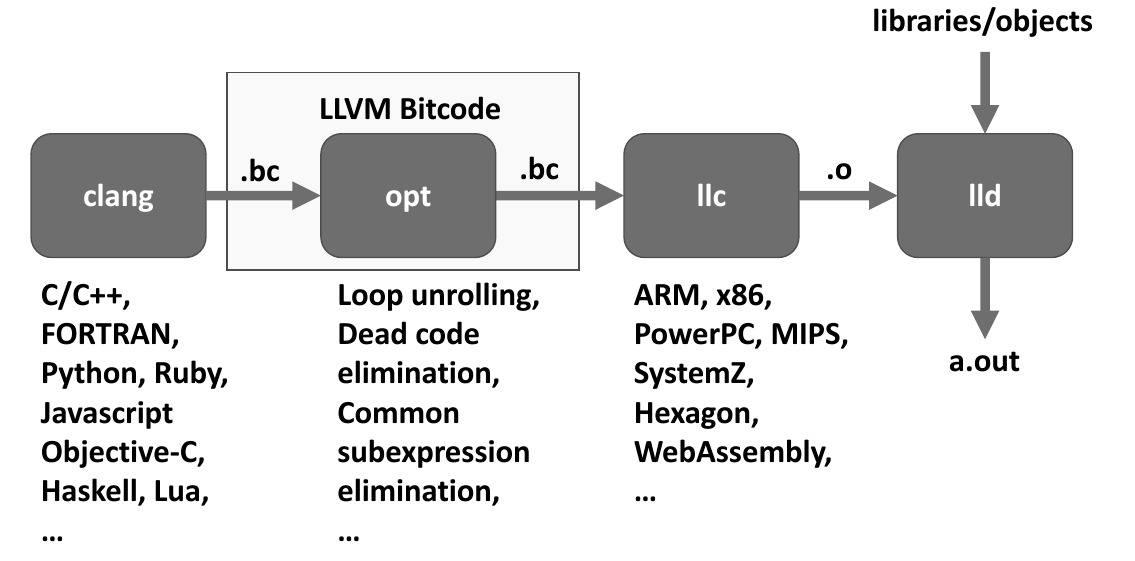
\includegraphics[scale=0.35]{LLVMcompiler.jpg}}
    }
    \caption{Various stages of compilation using Clang}
    \label{fig:LLVMcompiler}
\end{figure}

\section{Common Clang/LLVM Commands}
\label{sec:CommonClangLlvmCommands}

In each of the following commands, an optional output file can be specified using 
\texttt{'-o'} flag.
\begin{itemize} \tightlist
  \item \texttt{'clang hello.c'} - Compiles \textit{hello.c}.
  \item \texttt{'clang++ hello.cpp'} - Compiles \textit{hello.cpp}.
  \item \texttt{'clang -emit-llvm -S hello.c'} - Gives LLVM IR corresponding to \textit{hello.c} in text format file \textit{hello.ll}.
  \item \texttt{'clang -emit-llvm -c hello.c'} - Gives LLVM IR corresponding to \textit{hello.c} in binary bitcode format file \textit{hello.bc}.
  \item \texttt{'llvm-as hello.ll'} - Converts \textit{hello.ll} to \textit{hello.bc}.
  \item \texttt{'llvm-dis hello.bc'} - Converts \textit{hello.bc} to \textit{hello.ll}.
  \item \texttt{'lli hello.bc'} - Directly executes \textit{hello.bc}.
  \item \texttt{'lli hello.ll'} - Directly executes \textit{hello.ll}.
\end{itemize}

\noindent \textbf{NOTE} - Sometimes Clang/LLVM version information is also 
required for running the commands - \texttt{'clang-8', 'clang++-8, 'llvm-as-8', 'llvm-dis-8', 'lli-8'} etc.

\section{Working with Clang/LLVM}
\label{sec:WorkingWithClangLlvm}

This project is done on \textbf{Ubuntu 19.10} operating system using 
\href{https://clang.llvm.org/}{Clang} version 8.0.1 and 
\href{https://llvm.org/}{LLVM} version 8.0.1. The instructions 
mentioned here are verified to work on the same.

\subsection{Installing Clang}
\label{subsec:InstallClang}
First install \href{https://clang.llvm.org/}{Clang} using 
\texttt{'sudo apt-get install'} command. Also, make sure that its 
version is compatible with the version of LLVM to be used.
\smallbreak \noindent \textbf{NOTE} - Install Clang-8 (using 
\texttt{'sudo apt-get install clang-8'}) for working with LLVM-8.0.1.

\subsection{Building LLVM from source}
\label{subsec:BuildingLLVMFromSource}

Before proceeding make sure that \textbf{cmake} is installed on the 
system. For any further help on building LLVM from source, see 
\href{https://llvm.org/docs/CMake.html}{the LLVM documentation page}.

\begin{itemize} \tightlist
    \item First download the LLVM source code from 
    \href{http://releases.llvm.org/download.html}{LLVM download page} 
    or use \href{https://github.com/llvm/llvm-project/releases/download/llvmorg-8.0.1/llvm-8.0.1.src.tar.xz}{this link}
    to download source code for LLVM-8.0.1. 
    \item Extract the LLVM source from the tar-package, at some 
    preferable location. The root folder of the extracted source 
    will now be referred to as \texttt{LLVMsrc}.
    \item Create a new directory, which would be used for building 
    the LLVM source. This directory would be referred to as 
    \texttt{LLVMbuild}.
    \item Run \texttt{'cmake LLVMsrc'} from the \texttt{LLVMbuild} 
    directory. CMake will detect the development environment, perform 
    a series of tests, and generate the files required for building 
    LLVM. 
    \item Run \texttt{'cmake -{}-build .'} from the \texttt{LLVMbuild}
    directory to build the source.

    \textbf{NOTE} - This step might take hours to finish. Also, 
    building has very high memory requirements so it might also fail. 
    In this case repeat the last step and \textit{cmake} would detect 
    the packages it has already built in the previous run, and start 
    from where it was interrupted.
\end{itemize}
        
\subsection{Writing a Pass}
\label{subsec:WritingAPass}
A \textbf{pass} is a program that takes an LLVM IR as input and transforms it
generating a new IR. This new IR can be optimised version of the input or some 
modified version suitable for other tasks. Sometimes a pass only analyses 
the IR without modifying it.
\bigbreak \noindent This section explains how to create a simple pass named \textbf{HelloPass}.
\begin{itemize} \tightlist
    \item Create directory \textit{'LLVMsrc/lib/Transforms/HelloPass'}. This directory will contain files related to the pass.
    \item Create a new file named \textit{helloPass.cpp} inside \textit{HelloPass} directory. This file will contain the code for the pass which is given below.
        \begin{lstlisting}
#include "llvm/ADT/Statistic.h"
#include "llvm/IR/Function.h"
#include "llvm/Pass.h"
#include "llvm/Support/raw_ostream.h"
using namespace llvm;

namespace {
  struct helloPass : public FunctionPass {
    static char ID;
    helloPass() : FunctionPass(ID) {}

    bool runOnFunction(Function &F) override {
      errs() << "Function Name: ";
      errs().write_escaped(F.getName()) << '\n';
      errs() << "===================================================\n";
      for(auto bb = F.begin(); bb != F.end(); bb++){
        errs() << "\tBasicBlock Name = " << bb->getName() << "\n";
        errs() << "\tBasicBlock Size = " << bb->size() << "\n";
        for(auto i = bb->begin(); i != bb->end(); i++){
          errs() << "\t" << "Instruction: " << *i << "\n";
          errs() << "\t" << "OpCode: " << i->getOpcode() << "\n";
          errs() << "\t" << "OpCodeName: " << i->getOpcodeName() << "\n";
          errs() << "\t" << "IsBinaryOp: " << i->isBinaryOp() << "\n";
          errs() << "\t" << "IsCommutative: " << i->isCommutative() << "\n";
          errs() << "\t" << "IsAssociative: " << i->isAssociative() << "\n";
        }
        errs() << "\n\n";
      } 
      return false;
    }
  };
}
char itrinstBB::ID = 0;
static RegisterPass<helloPass> X("hello", 
                                 "Iterates instructions in a function");
        \end{lstlisting}
    The above code contains a \textbf{function pass} - which means the 
    pass is run on every function defined in a file. Using 
    iterators it traverses each basic block of the function, and 
    for each basic block, it traverses each instruction and 
    prints the details of the instruction - like its opcode, 
    whether it is commutative and associative etc.\\
    \textbf{Important} - Notice the first argument \textbf{hello} 
    which is passed in the last line while registering the pass. 
    This argument will be passed as a flag to the 
    \textbf{HelloPass} pass when the function-pass defined inside 
    \textbf{helloPass} structure (the template arguments in the last line)
    is to be executed.
    \item Create a file named \textbf{CMakeLists.txt} in the same 
    HelloPass dirctory. This file will be used by \textbf{make} when 
    building the pass.
        \begin{lstlisting}
add_llvm_library( LLVMhelloPass MODULE
  helloPass.cpp
  PLUGIN_TOOL
  opt
)
        \end{lstlisting}
        \textit{LLVMhelloPass} in the first line specifies the 
        filename (without *.so extension) inside \textit{'LLVMbuild/lib/'}
        directory, which will contain the pass when built. 
        \textit{helloPass.cpp} in the second line specifies the file 
        which contains the source code for the pass.
    \item Add the following line to the file 
    \textit{'LLVMsrc/lib/Transforms/CMakeLists.txt'}
        \begin{lstlisting}
add_subdirectory(HelloPass)
        \end{lstlisting}
    This is the name of folder which contains the files related to the pass 
    and will also be used by \textbf{make} while building.

\end{itemize}

\textbf{NOTE} - More detailed tutorial on writing a pass can be found 
\href{http://llvm.org/docs/WritingAnLLVMPass.html#quick-start-writing-hello-world}{here}.

\subsection{Running the pass}
\label{subsec:RunningThePass}
\begin{itemize} \tightlist
    \item Rebuild the LLVM source so that it includes the new
    pass that was added. For this change current directory to \textit
    {LLVMbuild} and run \texttt{'make'}.
    \item Now run the pass on a binary bitcode file \textit{source.bc}, 
    containing an LLVM IR as \\
    \texttt{'./bin/opt -load ./lib/LLVMhelloPass.so -hello source.bc -o sourceN.bc'}.\\
    The pass can also be run on a \texttt{'*.ll'} file in a similar way.
    
  \end{itemize}
  
\noindent \textbf{NOTE} - \texttt{'LLVMhelloPass'} is the same name that was
specified in the \textit{CMakeLists.txt} file of the pass folder. Also, 
\texttt{'-hello'} flag is the name by which the pass was registered.
